\chapter{Project Development}
	
In each of the previous chapters I have explored different aspects of the fields of home automation and voice assistance from a 
theoretical point of view, from their definition to smaller details, including additional explanations about a specific home automation 
system, openHAB.

At this time, I think I have provided enough background to begin my case study: the building of a home automation controller. As I 
mentioned in the openHAB chapter, I will base my project on this system and build on it, as it accomplishes very well the main
requirements that I determined for this project.

In this chapter, I will detail the process that I have followed in order to develop this project, from its specification to the final result.

\section{Product Specification}
The first task to do is to define the product. What should a home automation system do? What do users expect it to do? How? All 
the answers to these questions can be clarified by following some processes that, although they do not completely answer them (we 
can see many failed projects from time to time), they provide a very clear and detailed specification from the beginning.

\subsection{Personas}
Creating personas is a common process applied to the product design and development process in order to help in making a user-centered
design, and it is applicable in this project in order to have a better idea of what would users expect from the final product.

A persona is a representation of a user, typically based off user research and incorporating user goals, needs, and interests.

In this project, I am going to use proto-personas, which are based on secondary research and the guess of who they should be designed 
for, as currently we do not have means and time for making true research-based personas (and it is not the main objective in this project).

After thinking about the main uses of this system and the people that would be interested on it, I have extracted these three personas, 
representing its main uses, although not the only ones. I have built them with the online platform Xtensio, and the figures
\ref{fig:persona-oswald-douglas}, \ref{fig:persona-anna-lahtinen} and \ref{fig:persona-rosario-vera} represent them.

I tried to extract a varied range of backgrounds, current situations, desires and worries. Oswald Douglas (figure 
\ref{fig:persona-oswald-douglas}) is a freelance technology blogger from Dallas, USA, that is very interested in the areas of home 
automation and Internet of Things. He is looking to automate his own home and write about his experience in his blog. He already has 
experience with technology, and this next step will not be too difficult for him. His interests are clear: to try cutting-edge technology 
in his own home and make the most of home automation.

Anna Lahtinen is a 16 year-old high school student from Lappeenranta, Finland. She is up to date on technology but she is not passionate 
about it. However, she heard about home automation and thinks that she could enjoy a better media experience with it. In addition, she 
thinks that adding smart color light bulbs to her bedroom would make it look more beautiful. However, she feels that there is a lack
of general information about devices and the set up and configuration of a home automation system. She thinks that the price
of it is too high as well.

Rosario Vera is an administrative from Vitoria-Gasteiz, Spain. She is 37 years old, is married and has two young children. She is not 
very familiar with technology, but she has heard about home automation in the news and thinks that it could fit her needs. Rosario
and her husband work outside home, and sometimes their children need to be alone at home. Home automation would provide more security
to the home and would allow them to have more spare time. Voice assistance would be helpful for their children when they are alone,
as it is a very easy and natural way to interact with technology. However, she is concerned about their privacy regarding these systems
and she thinks that companies should give more accessible explanations about it. In addition, she finds these systems difficult to use.

\begin{sidewaysfigure}
	\centering
	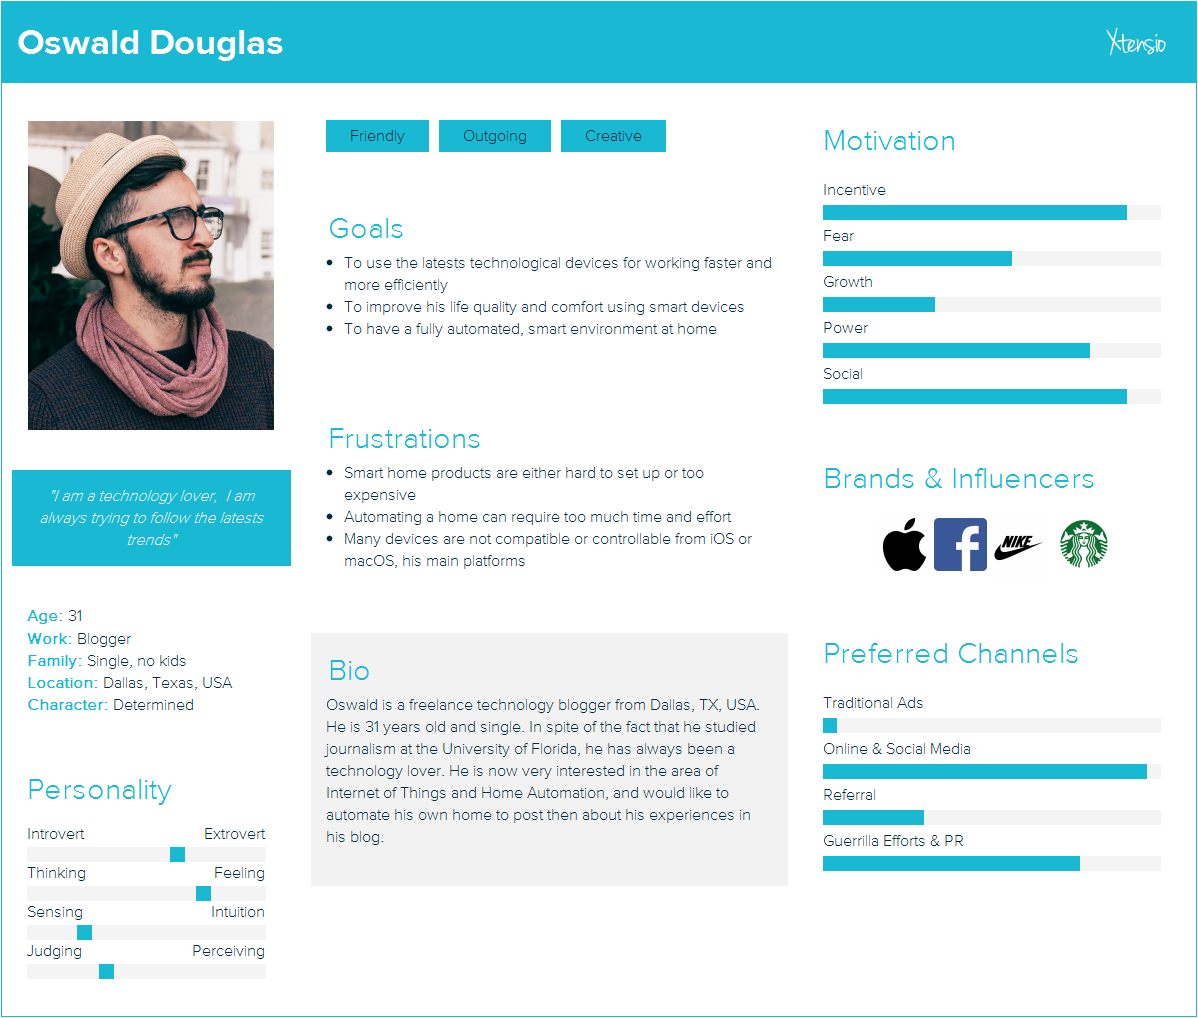
\includegraphics[width=0.65\textwidth]{images/Chapter_06/persona-oswald-douglas.png}
	\caption{Persona: Oswald Douglas}
	\label{fig:persona-oswald-douglas}
\end{sidewaysfigure}

\begin{sidewaysfigure}
	\centering
	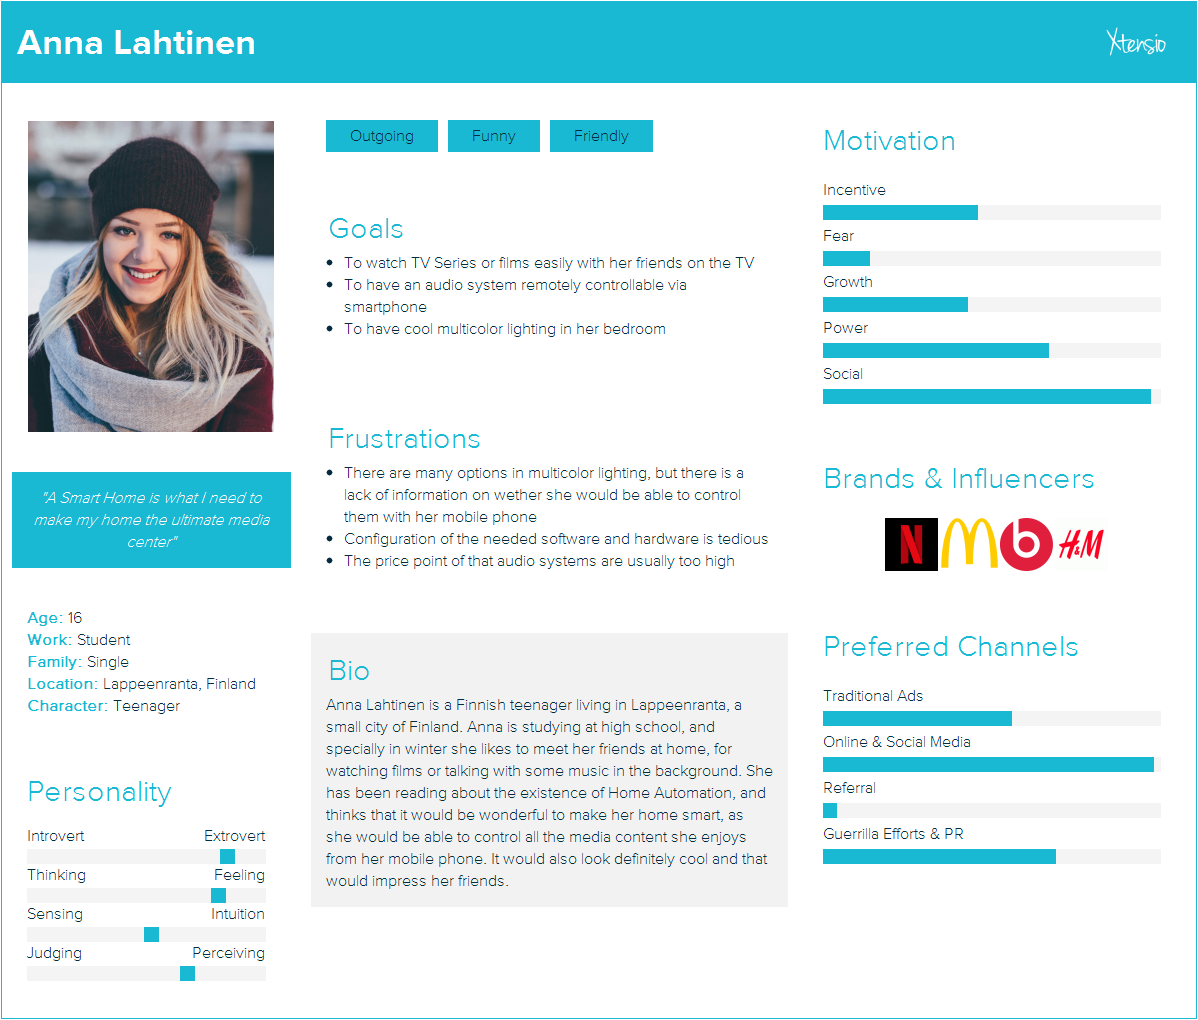
\includegraphics[width=0.65\textwidth]{images/Chapter_06/persona-anna-lahtinen.png}
	\caption{Persona: Anna Lahtinen}
	\label{fig:persona-anna-lahtinen}
\end{sidewaysfigure}

\begin{sidewaysfigure}
	\centering
	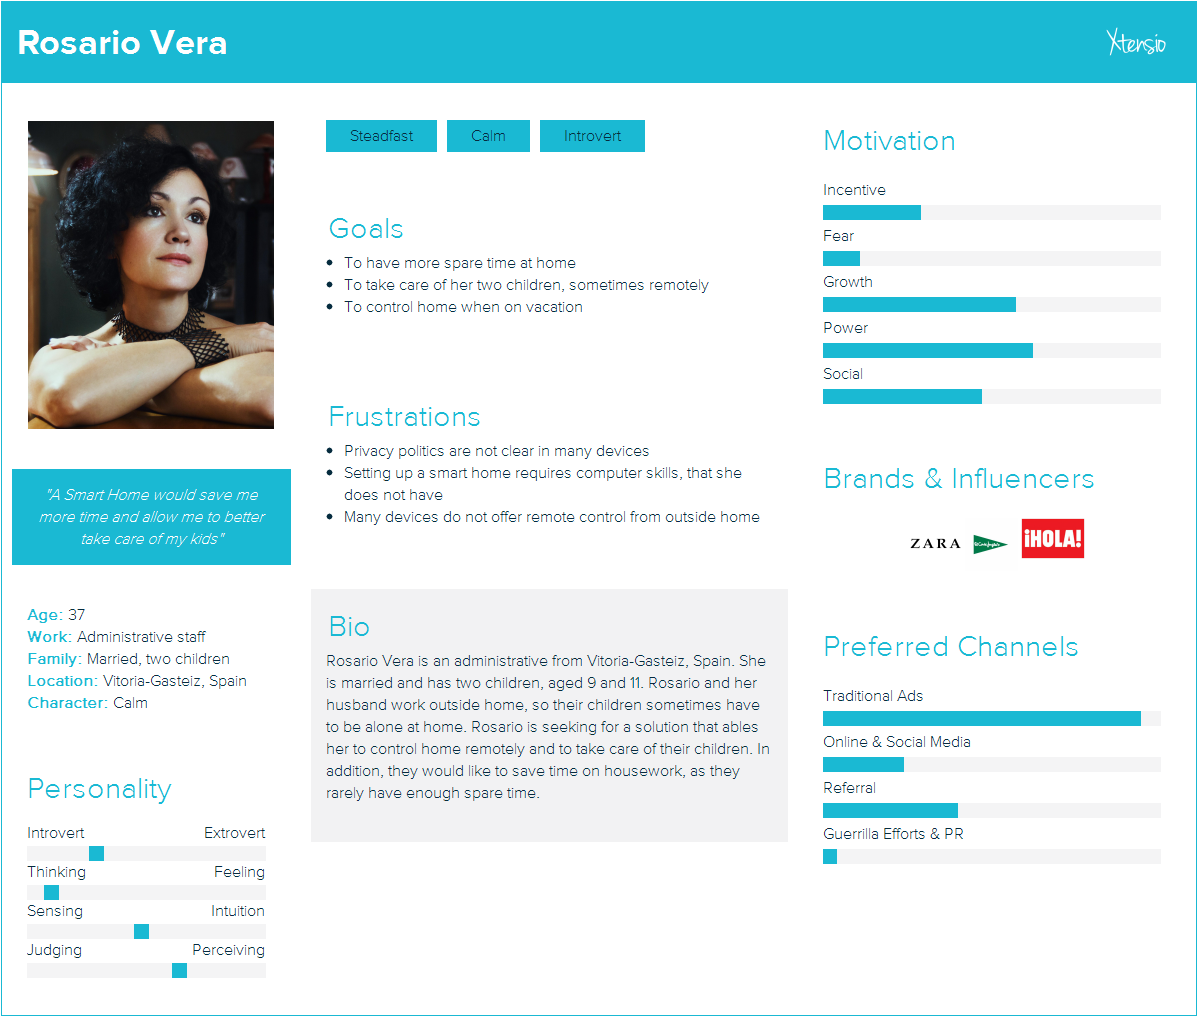
\includegraphics[width=0.65\textwidth]{images/Chapter_06/persona-rosario-vera.png}
	\caption{Persona: Rosario Vera}
	\label{fig:persona-rosario-vera}
\end{sidewaysfigure}

\subsection{Software Requirements Specification}
With the Software Requirements Specification (SRS), I try to describe the project to develop from a functional point of view, that is,
to determine the capabilities that the software system will have.

The domotic controller will be able to control all modern devices in our home, regardless of their maker and the technology they use.
It will provide an easy to use user interface and the ability to easily install, modify or remove the devices. It will also include natural
human-computer interaction through the voice. A more detailed specification of the requirements can be found in the subsections
below.

\subsubsection{Functional Requirements}
Functional requirements are a description of the facility or feature required. They deal with what the system should do or provide 
for users.\cite{sqaFunctionalNonFunctional}

\begin{itemize}
	\item \textbf{FR1}: The system will be able to retrieve automatically the status of the different properties of the elements.
	\item \textbf{FR2}: The system will be able to retrieve automatically data from its different data providers.
	\item \textbf{FR3}: The system will not need any operation to launch openHAB after it is powered on.
	\item \textbf{FR4}: The system will be able to turn itself off safely.
	\item \textbf{FR5}: The system will automatically detect new smart devices connected to the local network.
	\item \textbf{FR6}: The system will be able to detect the possible operations with each connected smart device. 
	\item \textbf{FR7}: The system will be able to operate with the connected devices according to the detected possible operations.
	\item \textbf{FR8}: The system will be able to tell the user in an understandable manner the current connection status for each
	device.
	\item \textbf{FR9}: The system will provide different user interfaces, so users can choose one between them, according to
	their needs.
	\item \textbf{FR10}: The user will be able to change the configuration of the system from a graphical user interface.
	\item \textbf{FR11}: The system will be manually configurable and modifiable using configuration files.
	\item \textbf{FR12}: The system will automatically include and configure new devices found in the network, after the user decides
	to add them.
	\item \textbf{FR13}: The user will be able to configure the name, display icon, IP and all possible aspects of the item directly from
	the user interface.
	\item \textbf{FR14}: The system will allow the user to make groups of items.
	\item \textbf{FR15}: The system will allow the user to add groups of items to other groups of items.
	\item \textbf{FR16}: The system will be modular and include a package system. Each package supports a set of devices.
	\item \textbf{FR17}: The package system will be accessible from the graphical user interface.
	\item \textbf{FR18}: The installation of packages will be done automatically after the user clicks on the install button.
	\item \textbf{FR19}: The removal of packages will be done automatically after the user clicks on the remove button.
	\item \textbf{FR20}: The system will maintain an updated and classified list of packages according to an external repository.
	\item \textbf{FR21}: The system will be manageable from external sources.
	\item \textbf{FR22}: The system will be accessible from external devices and from the Internet.
	\item \textbf{FR23}: The system will allow to have automation rules defined by the user.
	\item \textbf{FR24}: The voice assistant will allow to perform the main operations of each device in the system.
	\item \textbf{FR25}: The voice assistant will be able to answer in different languages.
	\item \textbf{FR26}: The voice assistant will be able to do power management tasks in the system, such as powering the system
	off or restarting the system.
	\item \textbf{FR27}: The voice assistant will be operable through mechanical methods or by voice.
	\item \textbf{FR28}: The users will be able to edit and adapt the functionalities of the voice assistant according to their needs.
	\item \textbf{FR29}: The voice assistant will provide spoken feedback if there has been an error performing the given command.
	\item \textbf{FR30}: The voice assistant will be able to print debug information in the command line if it is required.
\end{itemize}

\subsubsection{Non-Functional Requirements}
Non-functional requirements detail constraints, targets or control mechanisms for the new system. They describe how, how well or
to what standard a function should be provided.\cite{sqaFunctionalNonFunctional}

\begin{itemize}
	\item \textbf{NFR1}: The system, along with the voice assistant, will be installable in the Raspberry Pi.
	\item \textbf{NFR2}: The system and the voice assistant will provide a satisfactory response rate.
	\item \textbf{NFR3}: The user interfaces of the home automation system will be adaptable to the size and resolution of the
	user's screen.
	\item \textbf{NFR4}: The user interfaces will be made according to modern standards, like Material Design.
	\item \textbf{NFR5}: The home automation system will run in a local server, created in the machine which executes it.
	\item \textbf{NFR6}: In order to allow external connections, the home automation system will provide a REST API.
	\item \textbf{NFR7}: The system will provide secure access options.
	\item \textbf{NFR8}: The system must be available the 99\% of the time.
	\item \textbf{NFR9}: The system must be scalable.
	\item \textbf{NFR10}: The system must be recoverable in less than 45 minutes.
	\item \textbf{NFR11}: The cost of the system must me minimal.
	\item \textbf{NFR12}: The system must be interoperable with multiple devices.
	\item \textbf{NFR13}: The voice assistant will recognize English.
	\item \textbf{NFR14}: The voice assistant will be fast in its response. Therefore, its procedure for deciding a response will 
	be optimal.
	\item \textbf{NFR15}: The voice assistant will operate with the home automation system via REST, so it can be installed in a
	different computer than the one with the home assistant.
\end{itemize}
